\begin{blocksection}
\question Draw the environment diagram that results from running the code.

\begin{lstlisting}
def bar(f):
    def g(x):
        if x == 1:
            return f(x)
        else:
            return f(x) + g(x - 1)
    return g

f = 4
bar(lambda x: x + f)(2)
\end{lstlisting}

\begin{solution}[0.3in]
Output: 3 \newline
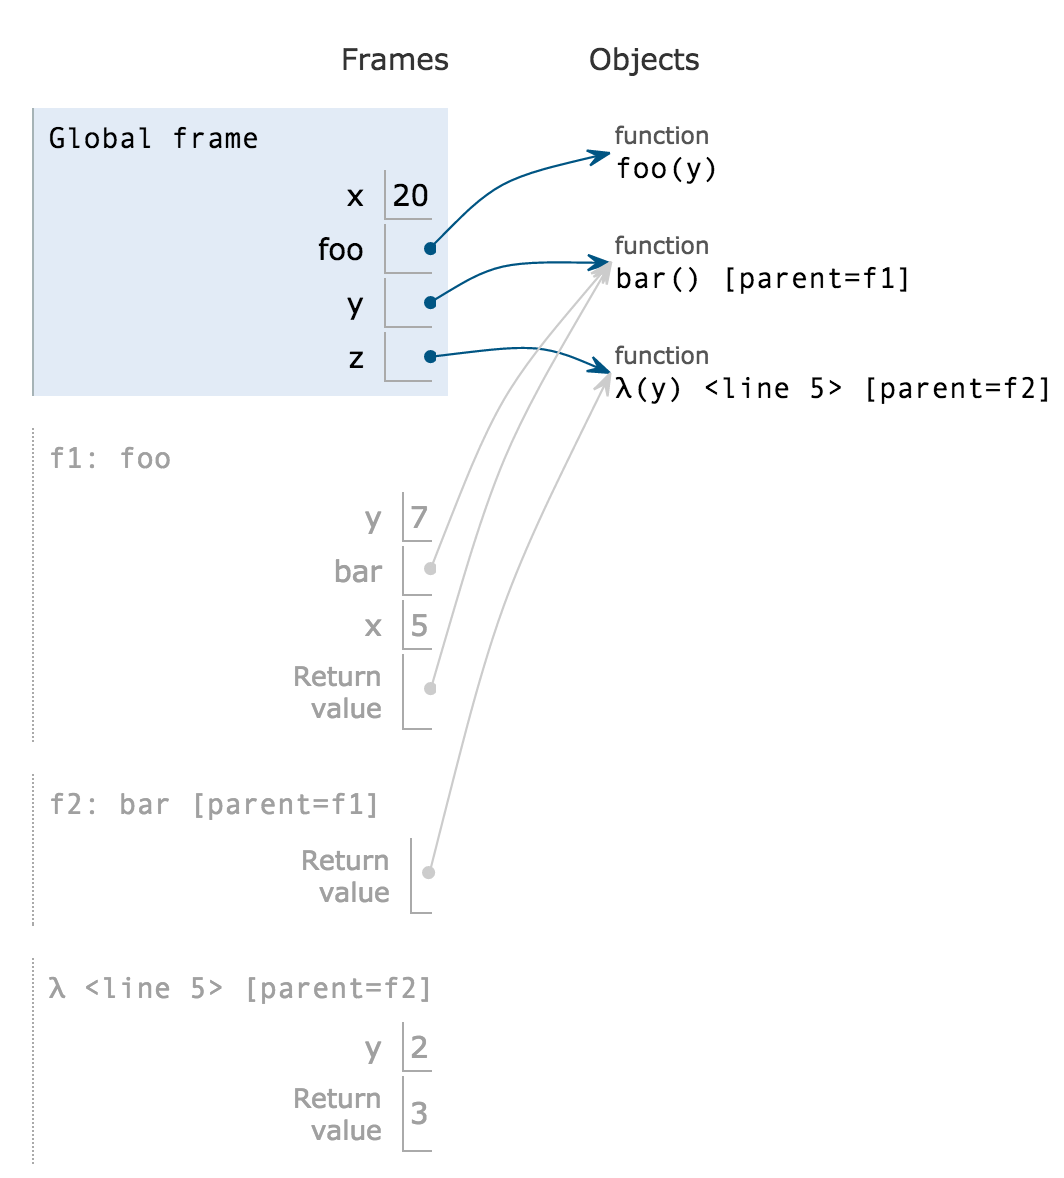
\includegraphics[scale=0.5]{foobar1.png}
\newline
\url{https://goo.gl/xD5kVE}
\end{solution}
\end{blocksection}
